\documentclass{article}
\usepackage[final]{nips_2017}
\usepackage[utf8]{inputenc} % allow utf-8 input
\usepackage[T1]{fontenc}    % use 8-bit T1 fonts
\usepackage{hyperref}       % hyperlinks
\usepackage{url}            % simple URL typesetting
\usepackage{booktabs}       % professional-quality tables
\usepackage{amsfonts}       % blackboard math symbols
\usepackage{nicefrac}       % compact symbols for 1/2, etc.
\usepackage{microtype}      % microtypography
\usepackage{graphicx}
\usepackage{amsmath}
\title{Automatic Code Generation Project Proposal}

\author{
  Lizi Ottens  \\
  Department of Computer Science\\
  Stanford University\\
  \texttt{lottens@stanford.edu}
  
  \and
  
  \textbf{Luis Perez} \\
  Department of Computer Science \\
  Stanford University \\
  \texttt{luis0@stanford.edu}
  
  \and
  
  \\
  \textbf{Sudharshan Viswanathan} \\
  Department of Computer Science \\
  Stanford University \\
  \texttt{viswans@stanford.edu}
}

\begin{document}
% \nipsfinalcopy is no longer used

\begin{center}

\includegraphics[width=3cm, height=0.7cm]{CS230}
\end{center}

\maketitle

\begin{abstract}
We propose developming a machine learning system for automatic code generation given a query string of text (eg, purpose of the program). The progress completed lies around three main axis: (1) refinement of problem statement, (2) in-depth analysis of CodeSearchNet dataset and (3) training of multiple exploratory baselines successfully.

Code used for baseline training and data-preprocessing is available on GitHub \footnote{See shared repository located at \href{https://github.com/kandluis/cs230}{https://github.com/kandluis/cs230}.}
\end{abstract}

\section{Problem Statement}
Automating even small parts of software development is an interesting research area \cite{survey} of machine learning that can save time for countless software engineers and resources for technology companies to invest into solving other more challenging problems. Automating code generation can take on many forms, from auto-completing lines of source code to generating lines of source code from comments, generating source code from UI images, or generating unit tests from source code. In this project, we aim to take incomplete lines of code as input and generate code to complete it.

\section{Background}
A primary challenge in code generation is that it’s still an active area of research, with many possible solutions and ongoing investigation \cite{structural_code_modeling}. State of the art solutions have not yet come close to automating basic tasks software engineers perform on a daily basis.

Other challenges include restricted language domains, complexity in evaluation results, etc. Specifically, while pre-trained models are trained on free-form language data, programming languages often utilize non-natural variable names, function names, and syntax with more structure \cite{structural_code_modeling}. Work in this area has focused on creating more structured models that take advantage of specific architectures \cite{treegen}. Other approaches involve restricting the output of the model to a CFG or DSL \cite{grammar_based}. A code generation model’s output must adhere to a very specific form in order to be syntactically correct.

Compilers/interpreters could be leveraged to provide a better form of feedback and hence can be used to create labelled data, but it is left to be seen how effectively we can leverage this feedback to aid the learning process.

\section{Methodology}
In this section we explain our methodology for multiple experiments and baselines proposed, as well as details on the training data and distribution.

\subsection{Data Analysis}
In this project, we are leveraging the \href{https://github.com/github/CodeSearchNet}{CodeSearchNet dataset} \cite{codesearchnet}. The dataset consists of 2 million (comment, code) pairs from open source libraries, ranging in languages from Python, Javascript, and PHP. Median code-length consists of 60-100 text tokens, with 95\% code-length of up to 350 tokens. Median documentation length consists of 10 text tokens. The distributions of methods and (comment, code) pairs across programming language are visualized in Figure \ref{fig:dist_methods}.

% TODO: Add visualization of training/dev/test dataset splits? 

\subsection{Baselines}
Figure \ref{fig:codesearchnet_arch} explains the general architecture of the baseline models from the CodeSearchNet task. We successfully trained and evaluated two baselines: Neural-Bag-Of-Words and an RNN-based baseline. See Section \ref{sec:results}.

Generally speaking, the baselines models take as input examples of (comments, code) pairs and learn to retrieve a specific code snippet. Each programming language has its own encoder network (see three columns to the right in Figure \ref{fig:codesearchnet_arch}, which are tasked with encoding a set of candidate code snippets. They are then combined through a dot product operation with the embedding generated by the query (docstring) encoder to produce a matrix comparison. 

The matrix diagonal serves as the scores of each query doc string/code snippet. Through this methodology, these baseline models are able to extract meaningful information and learn a joint distribution over the query and comment pairs. We train these models as a baseline since we believe they will be useful in the downstream task of code generation. The models are trained on the following loss function:

\begin{align}
    -\frac{1}{N}\sum_i \log \left( \frac{\exp(E_c(\textbf{c}_i^T)E_q(\textbf{d}_i))}{\sum_{j} \exp(E_c(\textbf{c}_j^T)E_q(\textbf{d}_j))}  \right)
    \label{eq:code_search_net_loss}
\end{align}

\section{Results}
\label{sec:results}
CodeSearchNet provides a good starting point as we are able to train different models on the input code streams. We trained a simple LSTM model as well as a neural bag of words model on a combination of all the available (code, documentation) pairs.

The Neural Bag of Words and LSTM CodeSearchNet baselines both report metrics in the same fashion. Below, we show the training curves, which correspond to the loss in Equation \eqref{eq:code_search_net_loss}.

Additionally, given that the baselines models for CodeSearchNet focus on code snippet retrieval, we also report the achieved mean reciprocal rank. The MRR is a statistic measure for evaluating any process that produces a list of possible responses to a sample of queries, ordered by probability of correctness. The reciprocal rank of a query response is the multiplicative inverse of the rank of the first correct answer: 1 for first place, $\frac{1}{2}$ for second place, $\frac{1}{3}$ for third place and so on. The mean reciprocal rank is the average of the reciprocal ranks of results for a sample of queries, as in Equation \eqref{eq:mrr}.

\begin{align}
    \text{MRR} = \frac{1}{|Q|}\sum_{i=1}^{|Q|} \frac{1}{\text{rank}_i}
    \label{eq:mrr}
\end{align}

\subsection{Neural Bag of Words Baselines}
This baseline consists of a simple encoder architecture which takes as input bag-of-words representation of the code and using a single neural network encodes these token representation into an embedding \cite{codesearchnet}. This baseline actually performs the best, achieving the lowest overall training and validation losses (see Figure \ref{fig:train_valid_neural_bow_model}) as well as the highest MRR on the validation set (See Figure \ref{fig:val_mrr_neuralbow}).

\subsection{Bi-directional RNN Model}
In this model, we employ the GRU cell \cite{gru_cell} to summarize the input sequence. This baseline performs significantly worse, suffering from what appears to be obvious over-fitting. In Figure \ref{fig:train_valid_neural_rnn_model}, we can see that while the training loss appears to plateau, the validation loss begins quickly climbing. While this behavior does not appear to affect the overall MRR achieved on the validation set, it's still clear that the model performs worse than the bag of words baseline as per Figure \ref{fig:val_mrr_rnn}.

\subsection{Code Generation with Char-RNN}
As both of the above baselines focus on understanding and extracting useful embedding for our overall task, our primary baseline consists of a straight-forward sequence-to-sequence model. Given that code typically does not consists of English words (but instead can have quite a varied syntax), our baseline model is a model which uses character level embedding, so it is character aware \cite{charrnn}.

Due to computational constraints, we train only on the Python subset of the data and only on 10\% of the total data available. For the char-rnn model \cite{charrnn}, this corresponds to around 50MB of raw text, or 78,357,395 characters with 1,618 distinct symbols. Figure \ref{fig:char_rnn_loss} shows the training and validation losses on the model. The loss is simply a softmax loss on the 1,618 characters for a sequence of length 128 (the model is trained on sequences of length 128 by default). Figure \ref{fig:char_rnn_perplexity} shows the perplexity, or the amount of meaninful information encoder. 

We include a sample generated from the best performing model for reference.
\begin{verbatim}
Downloads Dailymotion videos by URL. (x or pillares (if macks), style as a bool to you extner method instruxError,
       to oio instance of that Seir to be two categorical String to mandation :attr:`ColumnserverName(
                zr, j)
        dimensed_source
        also = ``axis``. Element. This repr_dures a substimcle of

        """
        code = item
    return self.filename
            restroxig, self.get_channels():
    """Get the function as firmap_list {1} and a :attracted_coordint: value of Time
    end_aes:
            target_ext = int(cmd_dict):
            # In data applicate horinad(string): the channel for decoded collfile
            Runnee network number of element. What you's associates py ch of List does request. Channels represented should be a TargetExcept the more notes

        ``index``.
def vert_event_notify_channel(self, infna=1)
                    elif trying.format(
        comps + ',' % (random) + 1,
            H.data:
            if list + lookbing.get('get_dict.get']}
\end{verbatim}

\section{Next Steps}
TODO


\bibliographystyle{unsrt}
\bibliography{references}

\newpage
\section*{Appendix and Figures}

\begin{figure}[!ht]
    \centering
    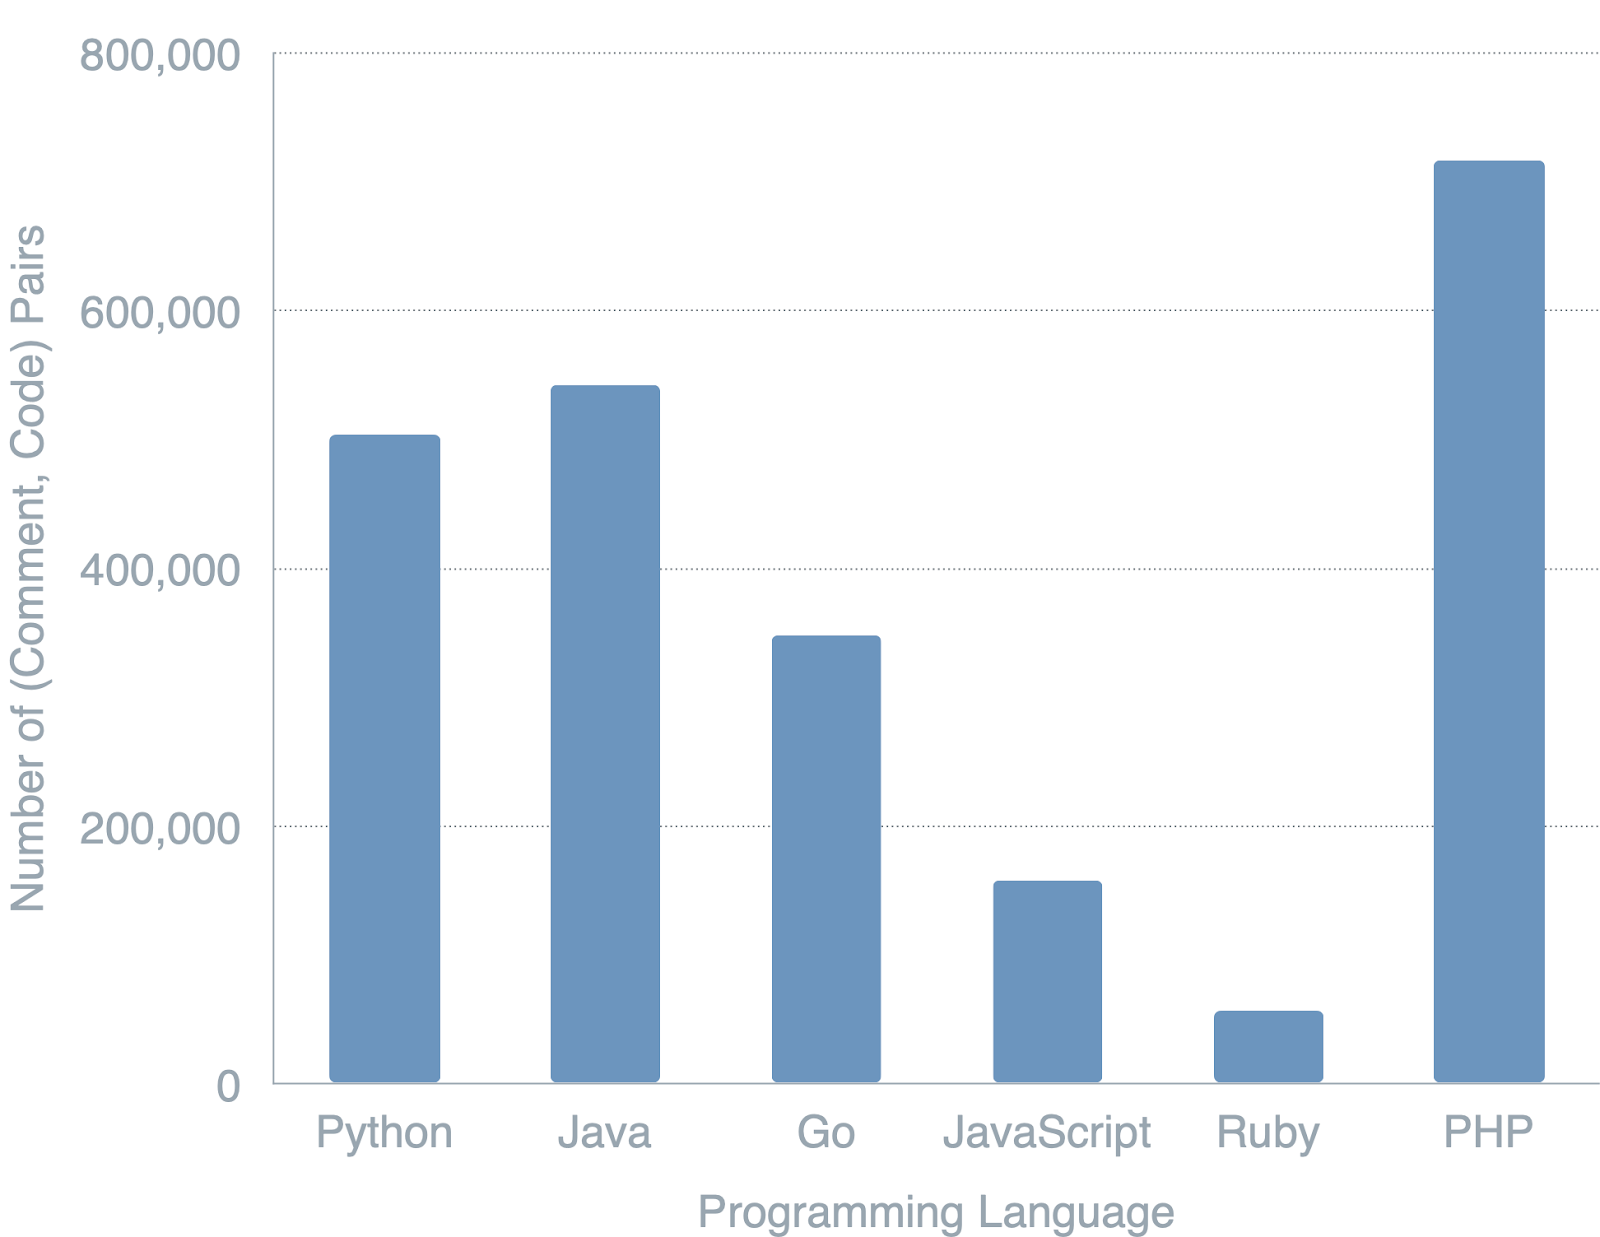
\includegraphics[scale=0.12]{figures/data_analysis/dist2.png}
    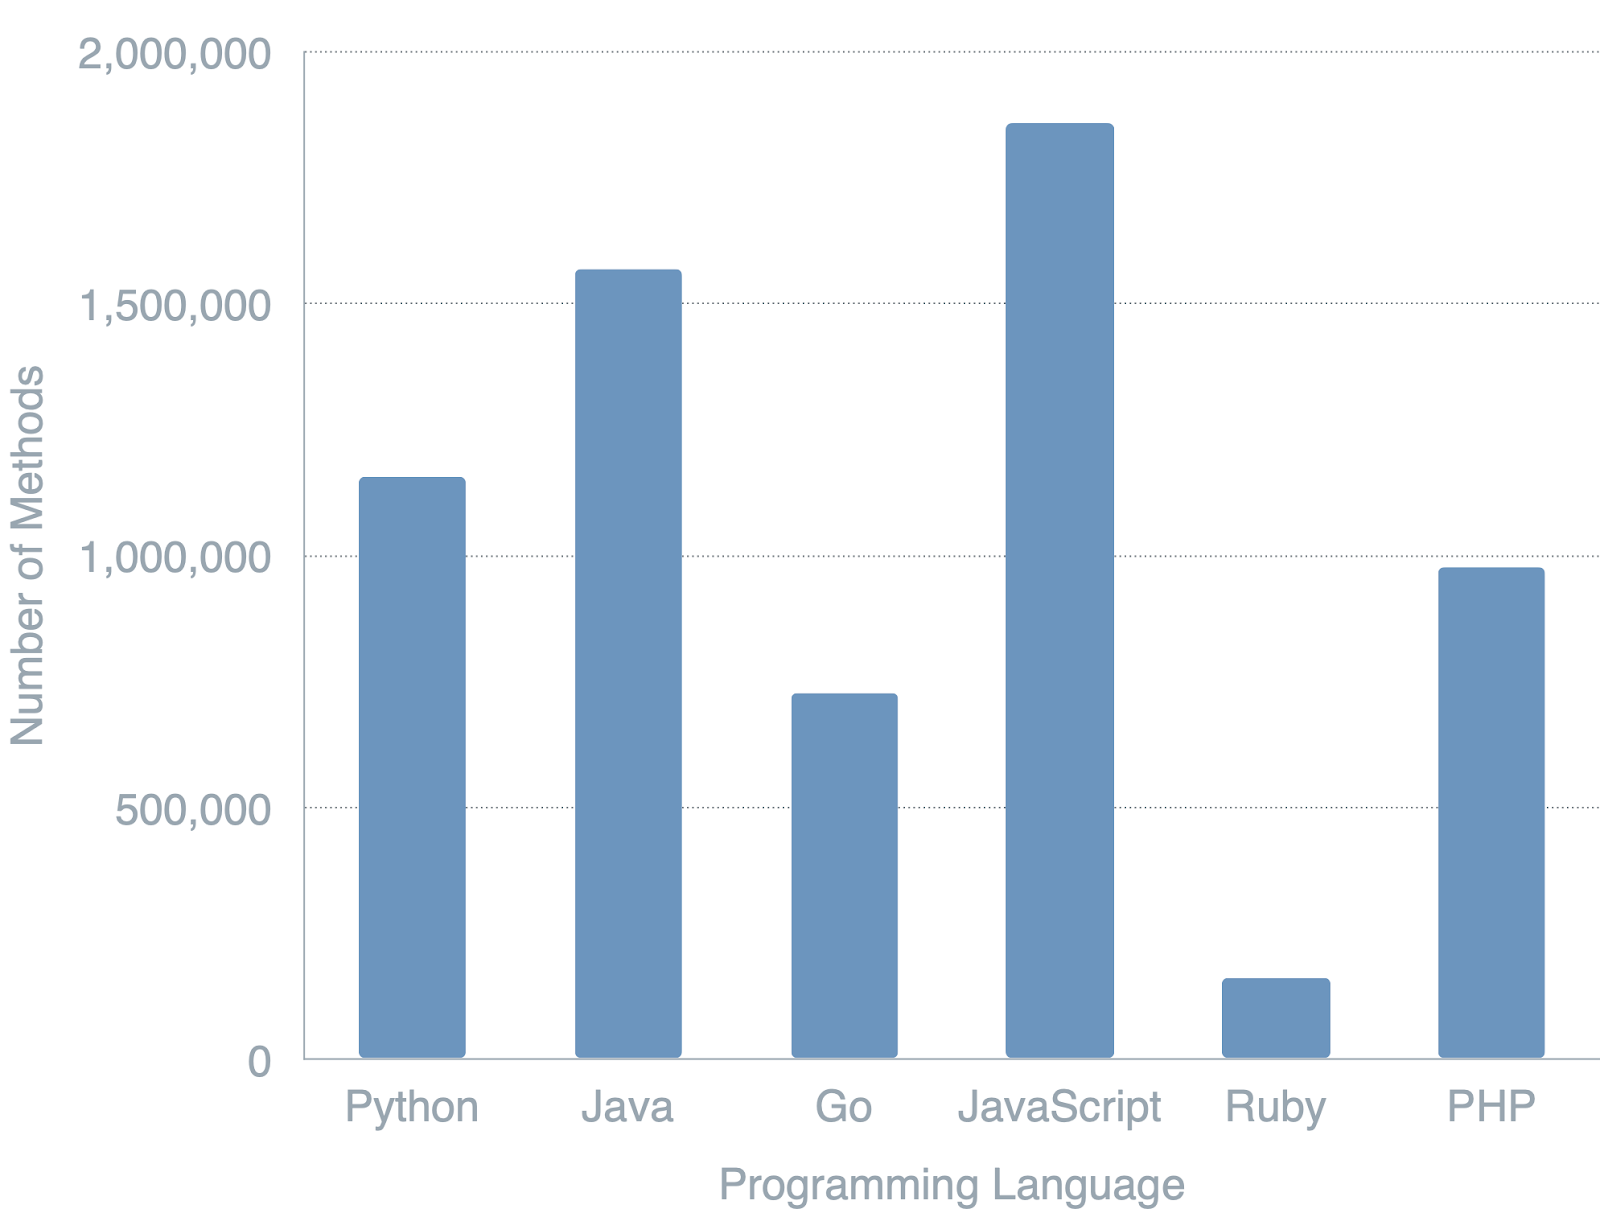
\includegraphics[scale=0.12]{figures/data_analysis/dists3.png}
    \caption{Histogram of the the number of (comment, code) pairs available in our dataset, as well as the number of unique function methods for each language.}
    \label{fig:dist_methods}
\end{figure}

\begin{figure}[!ht]
    \centering
    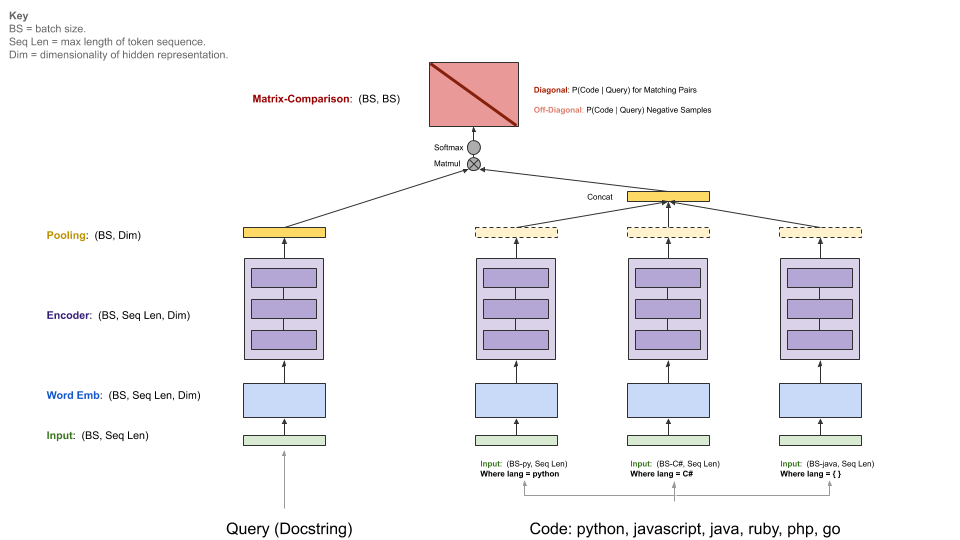
\includegraphics[scale=0.22]{figures/codesearchnet_arch.png}
    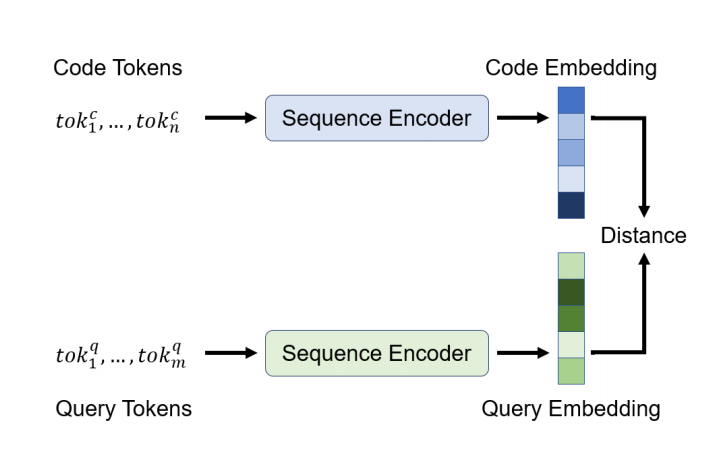
\includegraphics[scale=0.22]{figures/codesearchnet_approach.png}
    \caption{General CodeSearchNet architecture for all of our baselines. Each language is processed through different encoder mechanisms. The query encoder is shared (an NLP encoder), and the purpose of the CodeSearchNet tasks is to retrieve the most relevant code snippets subject to the natural language query.}
    \label{fig:codesearchnet_arch}
\end{figure}

\begin{figure}[!ht]
    \centering
    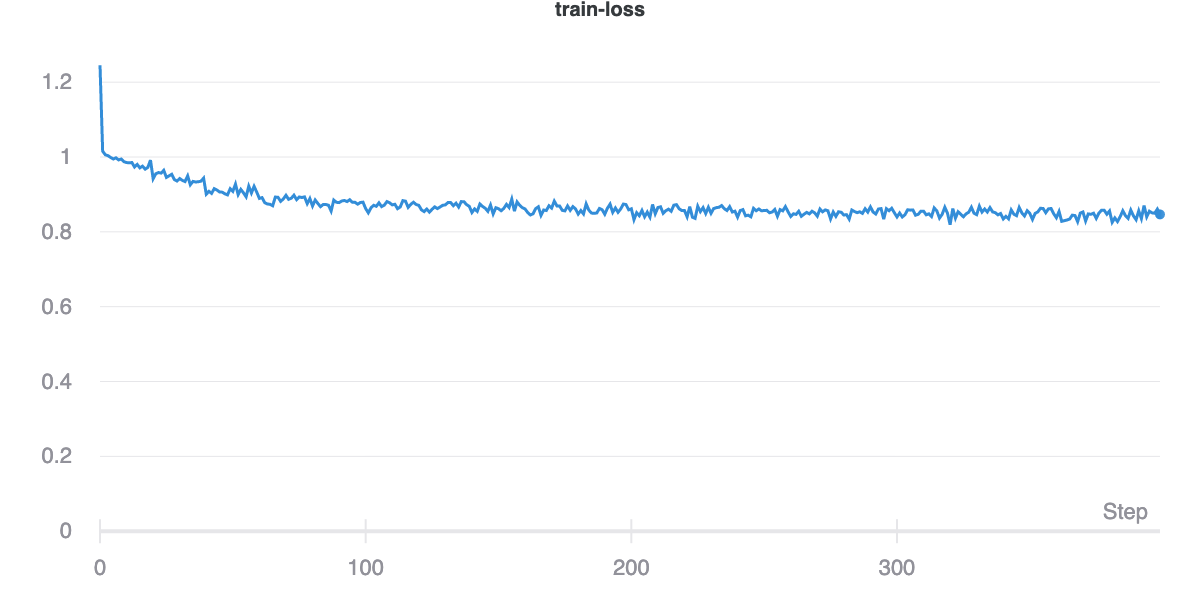
\includegraphics[scale=0.16]{figures/neuralbow/train-loss.png}
    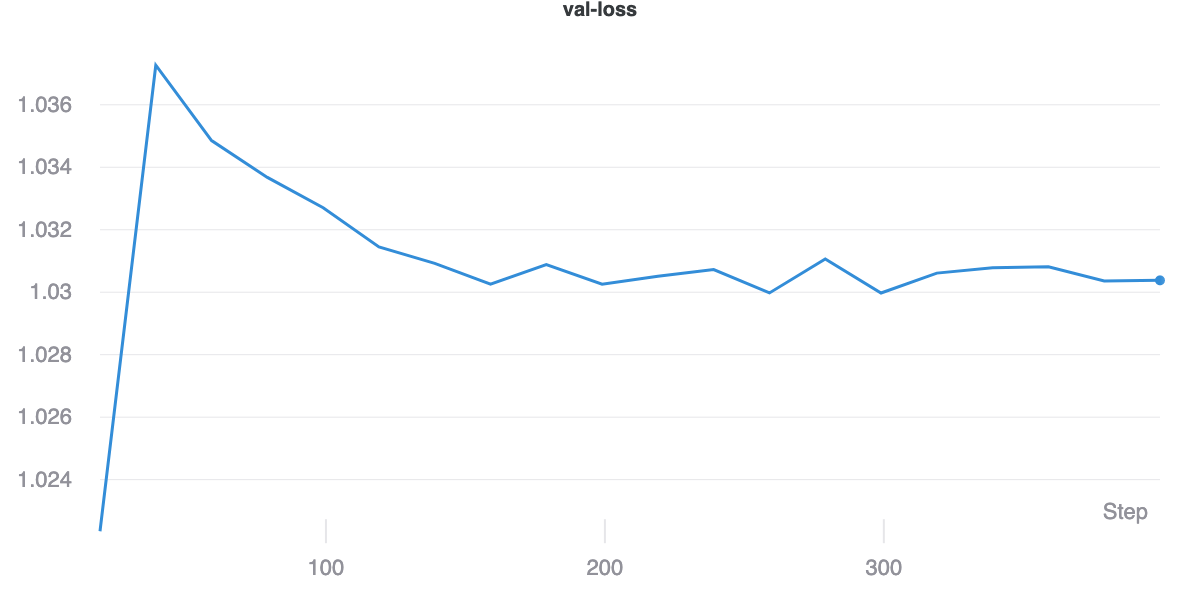
\includegraphics[scale=0.16]{figures/neuralbow/val-loss.png}
    \caption{Training and Validation losses for the Neural Bag of Words model in CodeSearchNet.}
    \label{fig:train_valid_neural_bow_model}
\end{figure}

\begin{figure}[!ht]
    \centering
    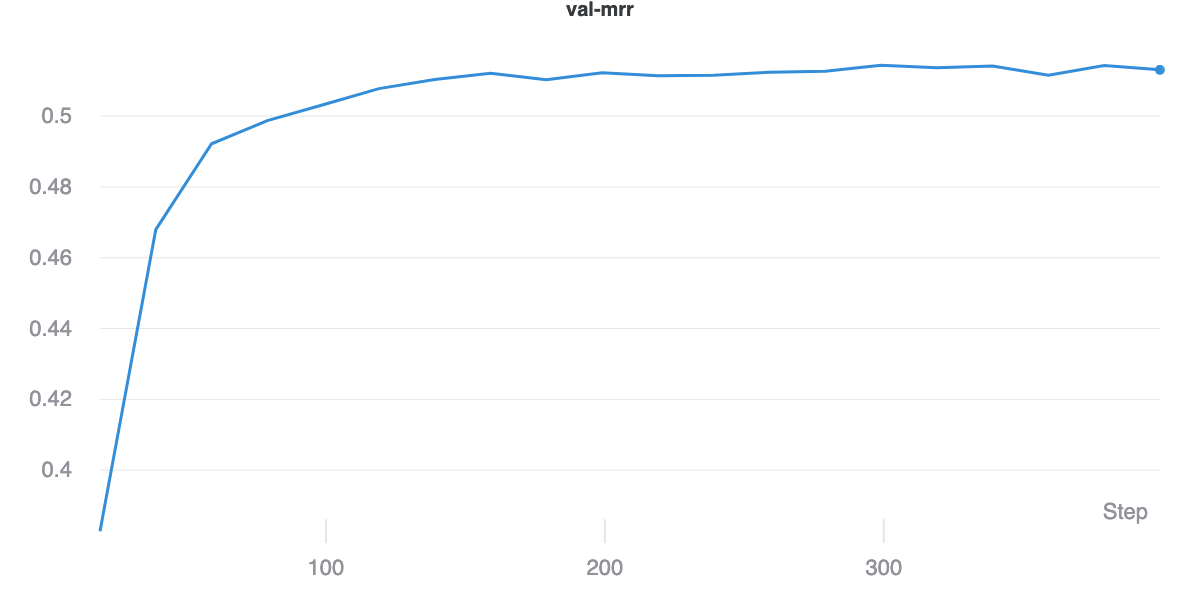
\includegraphics[scale=0.3]{figures/neuralbow/val-mrr.png}
    \caption{MRR on validation set for the baseline neural bag of words model in the CodeSearchNet Challenge.}
    \label{fig:val_mrr_neuralbow}
\end{figure}

\begin{figure}[!ht]
    \centering
    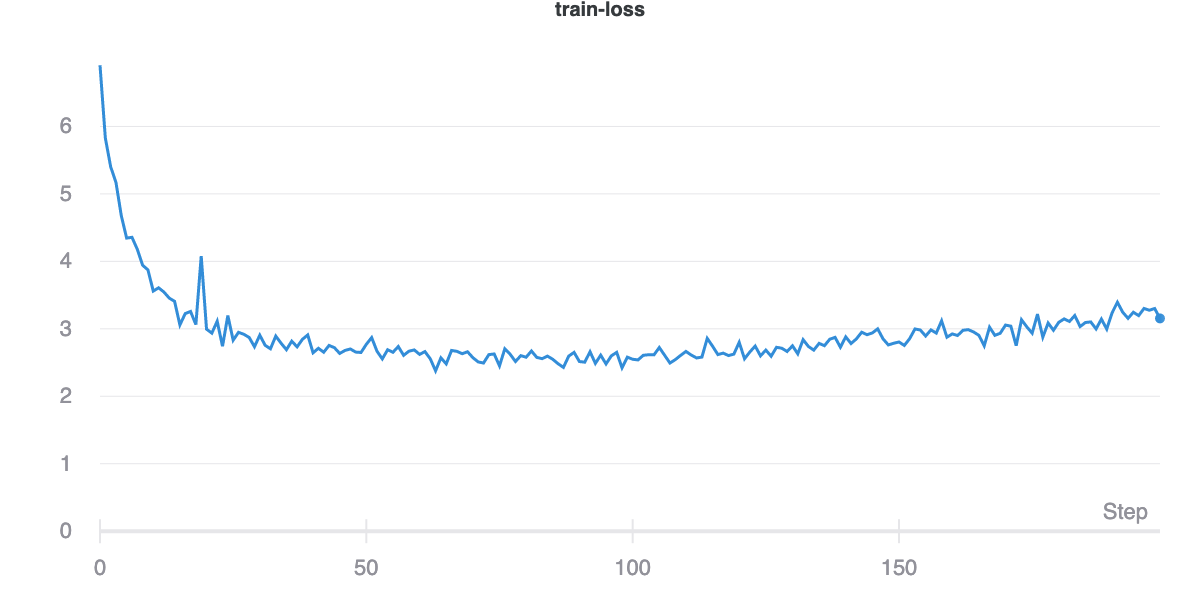
\includegraphics[scale=0.16]{figures/rnn/train-loss.png}
    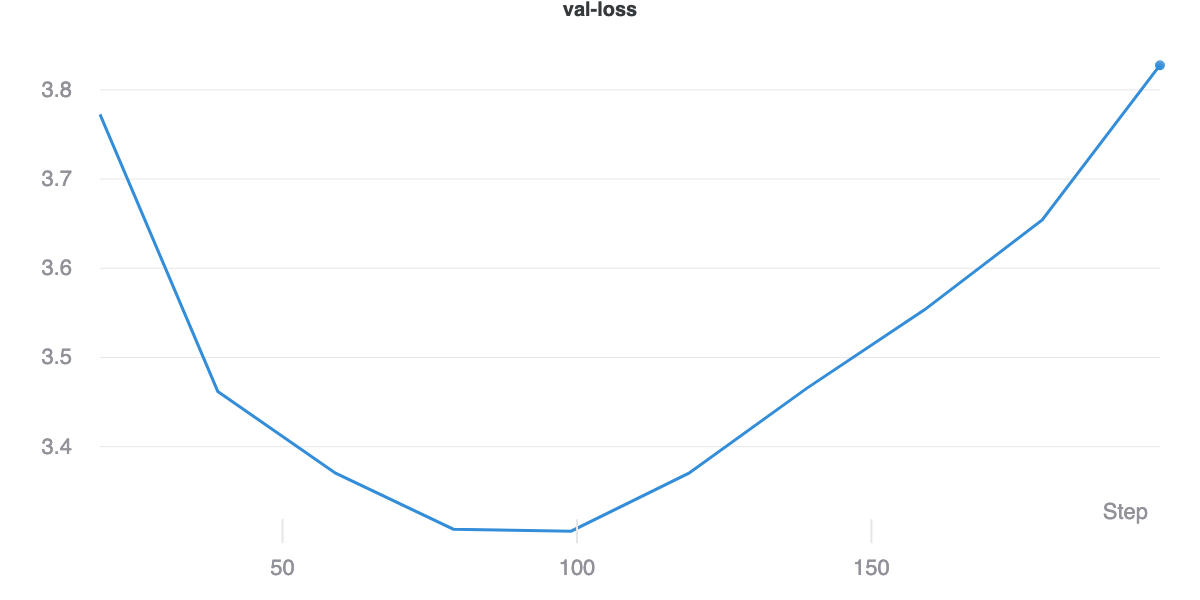
\includegraphics[scale=0.16]{figures/rnn/val-loss.png}
    \caption{Training and Validation losses for the RNN model in CodeSearchNet.}
    \label{fig:train_valid_neural_rnn_model}
\end{figure}

\begin{figure}[!ht]
    \centering
    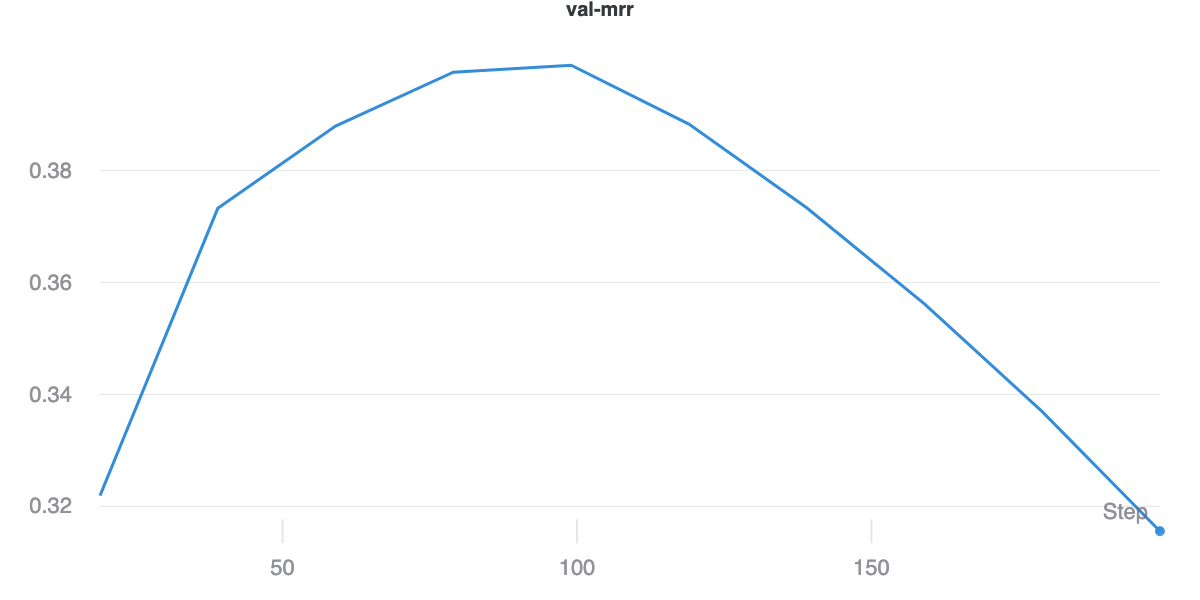
\includegraphics[scale=0.3]{figures/rnn/val-mrr.png}
    \caption{MRR on validation set for the baseline RNN in the CodeSearchNet Challenge.}
    \label{fig:val_mrr_rnn}
\end{figure}

\begin{figure}[!ht]
    \centering
    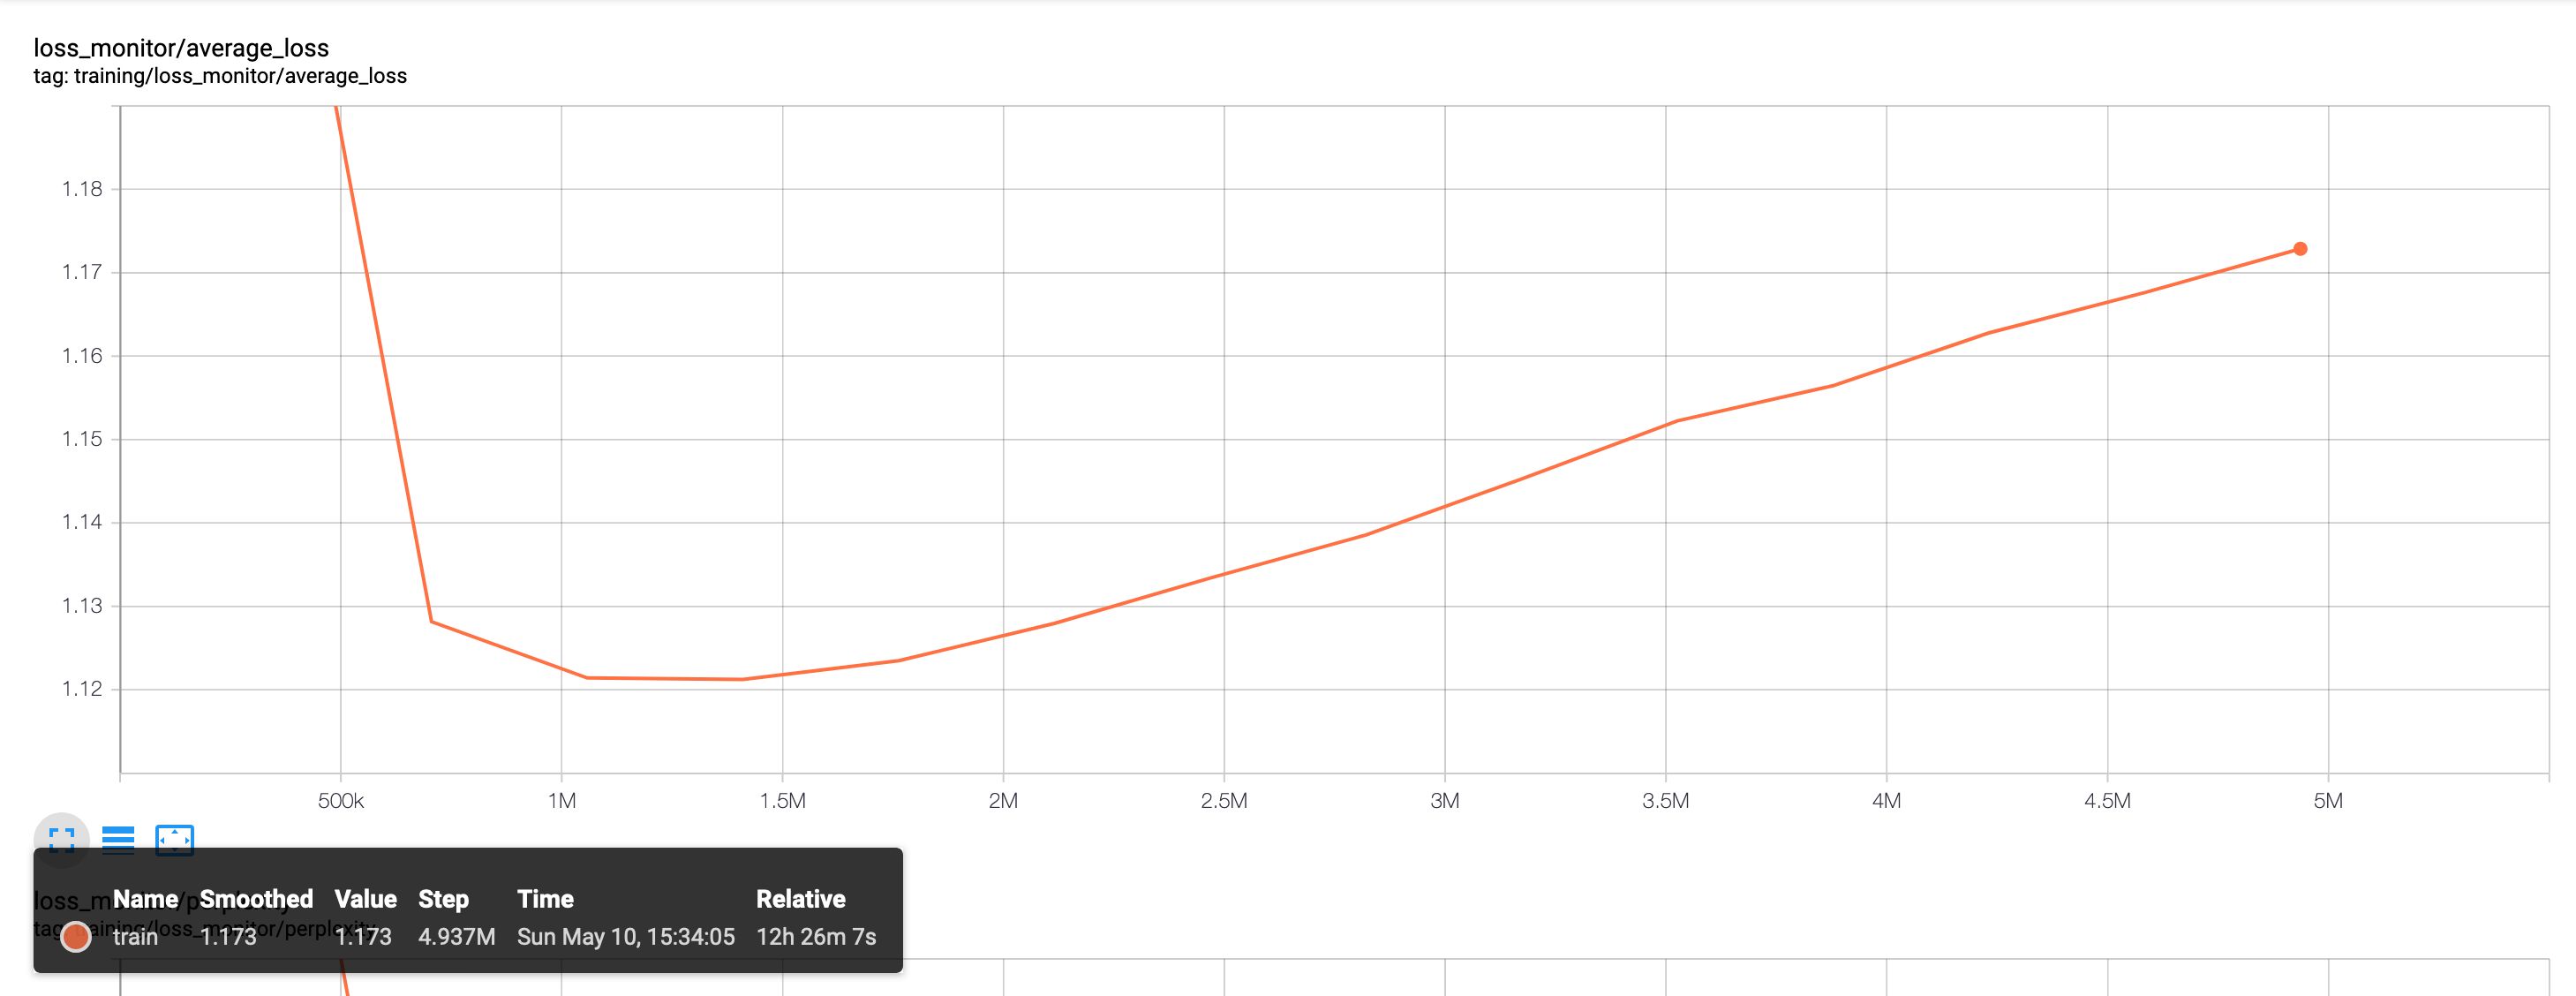
\includegraphics[scale=0.3]{figures/char-rnn/train_loss.png}
    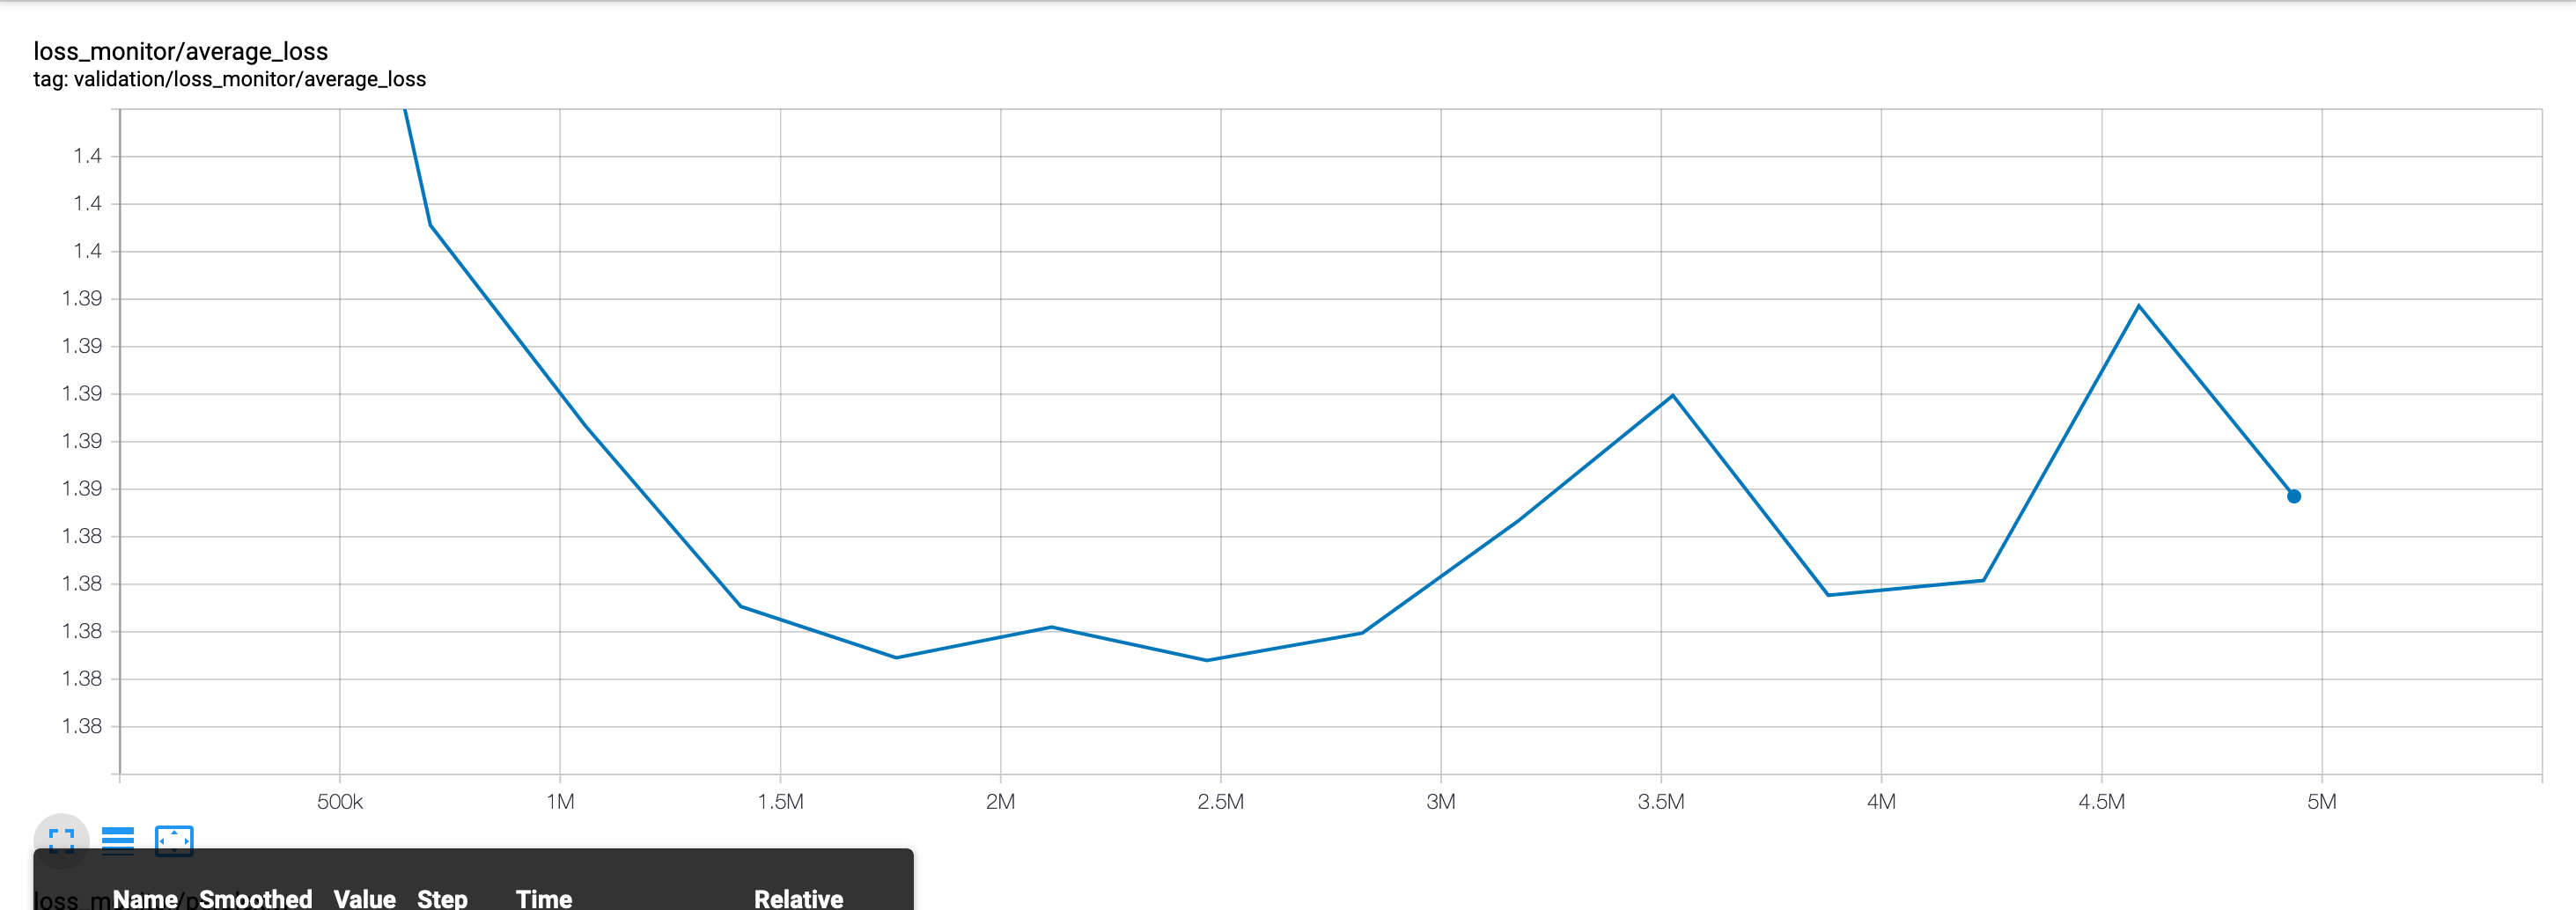
\includegraphics[scale=0.3]{figures/char-rnn/validation_loss.png}
    \caption{Training and Validation Losses on the Baseline Char-RNN Model. This is the cross-entropy loss over 128 predicted character sequence.}
    \label{fig:char_rnn_loss}
\end{figure}

\begin{figure}[!ht]
    \centering
    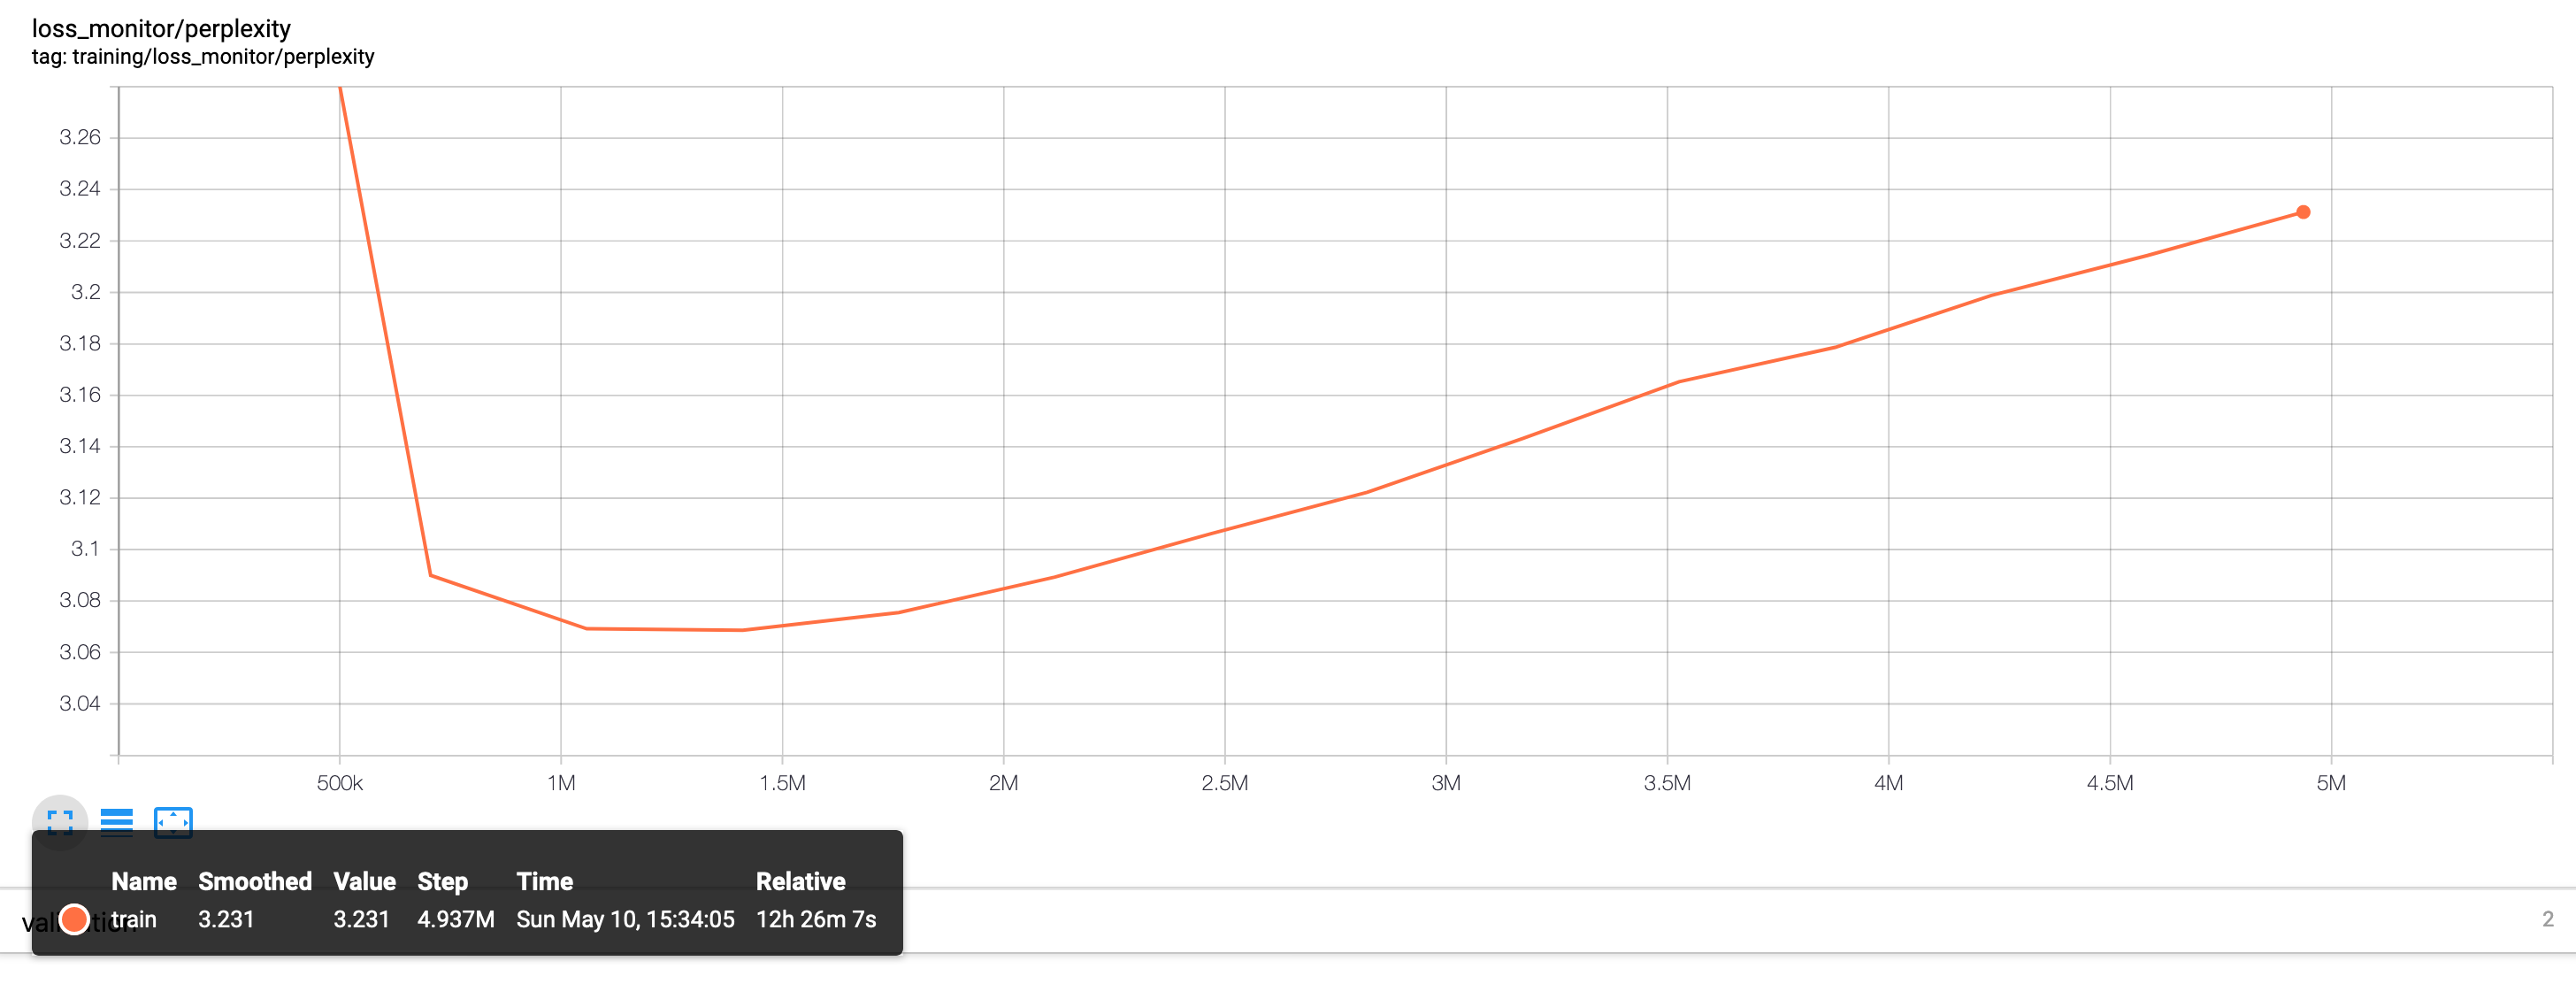
\includegraphics[scale=0.3]{figures/char-rnn/train_perplexity.png}
    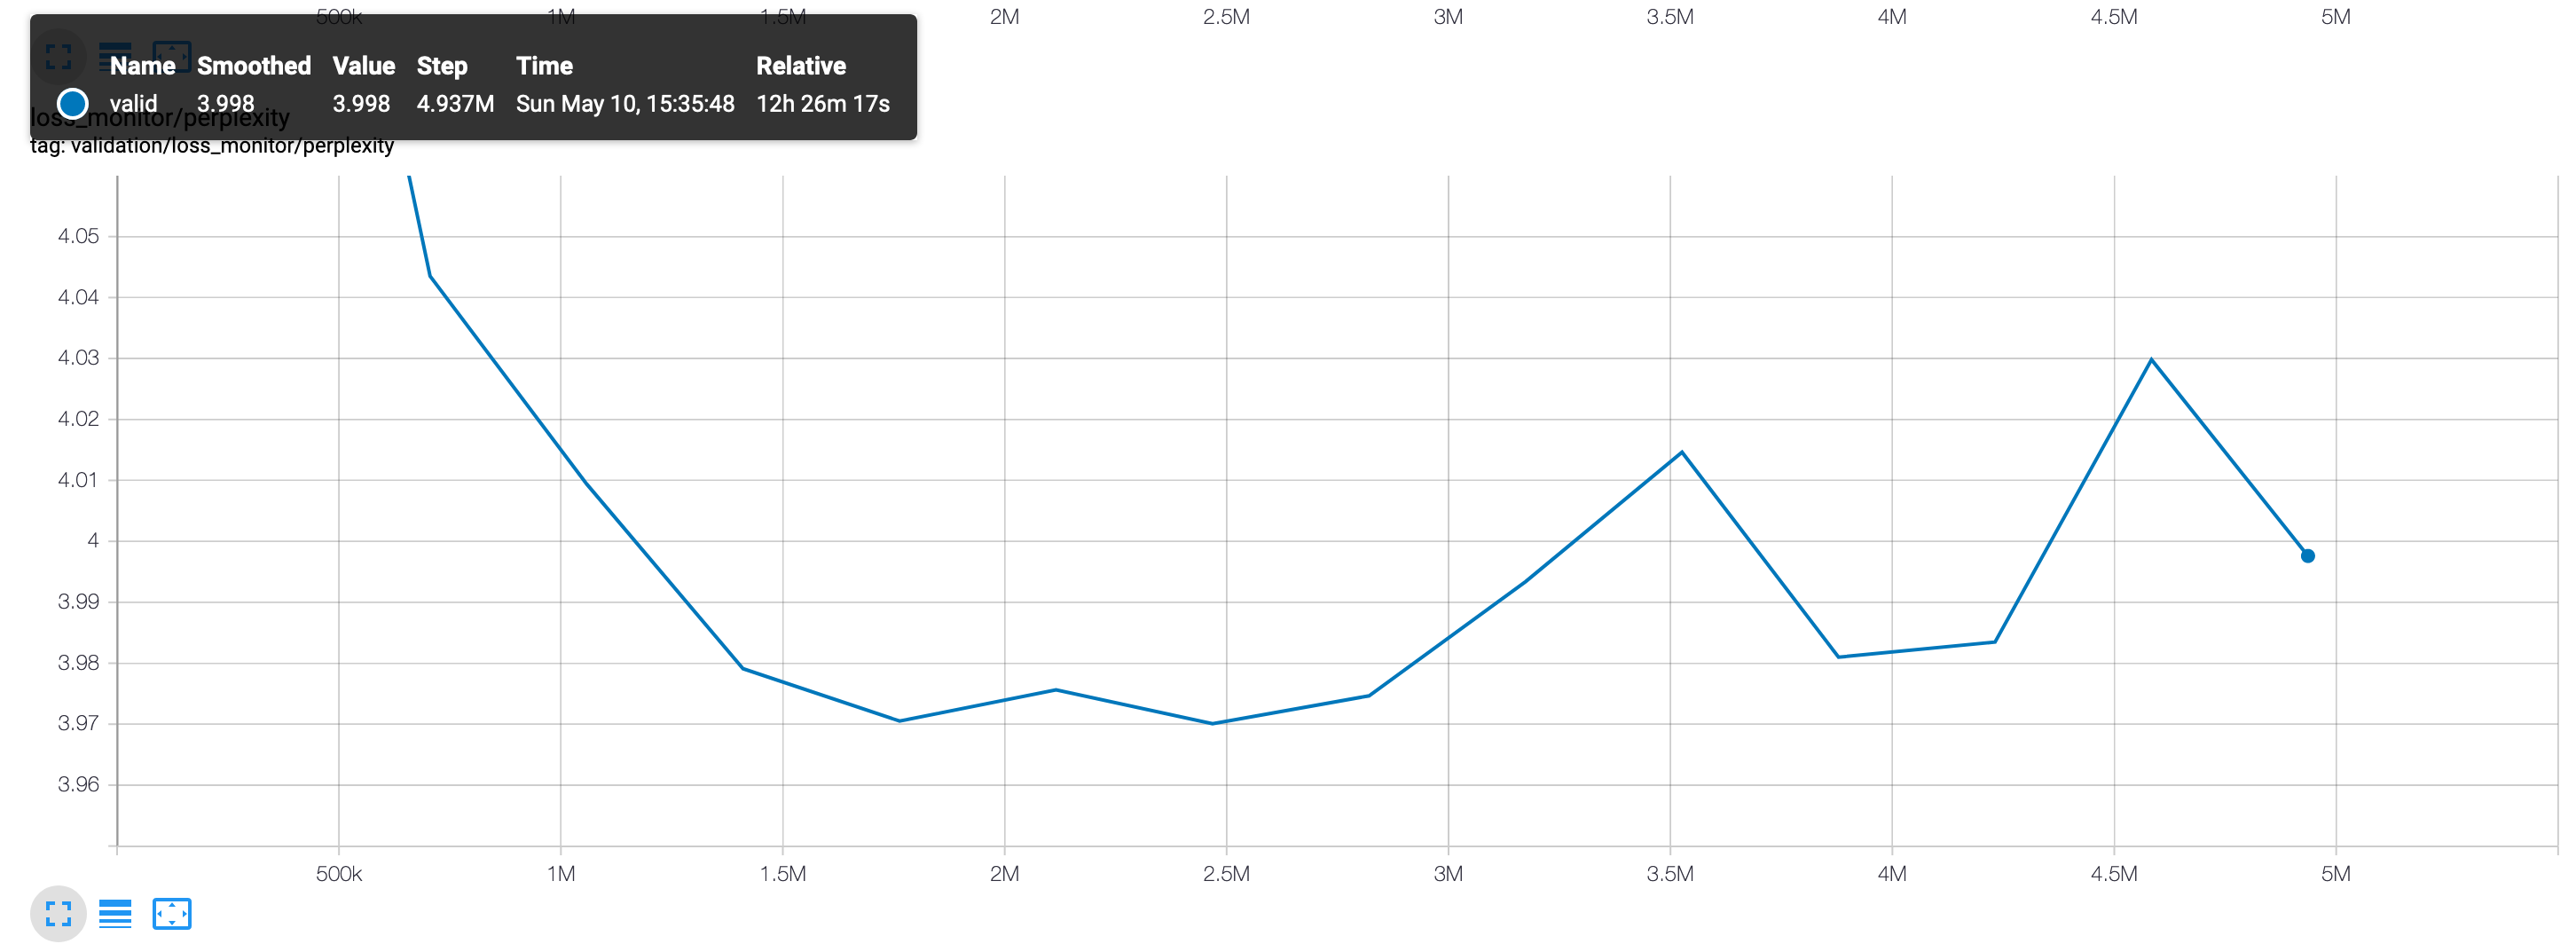
\includegraphics[scale=0.3]{figures/char-rnn/validation_perplexity.png}
    \caption{Training and Validation Perplexity on the Baseline Char-RNN Model. This is the cross-entropy loss over 128 predicted character sequence.}
    \label{fig:char_rnn_perplexity}
\end{figure}

\end{document}